%This is a sample thesis file for all CPP Math Grad Students to follow.  
% After downloading this file to your computer, save it with whatever name you wish.
% Then download the file    CPP.cls  and be sure to save it in the same folder where
% you saved this file.  Do NOT change the name of CPP.cls    
\documentclass{cpp}

% \usepackage{url}
\usepackage{hyperref}
\usepackage{amsthm}
\usepackage{amsmath}
\usepackage{amssymb}
\usepackage{latexsym}
\usepackage{verbatim}
\usepackage{graphicx}
\usepackage{float}
\usepackage{algorithm}
\usepackage[noend]{algpseudocode}
% \usepackage{pythonhighlight}

\usepackage[utf8]{inputenc}
\usepackage{listings}
\usepackage{xcolor}
\definecolor{codegreen}{RGB}{0, 128, 0}
\definecolor{codegray}{gray}{0.55}
\definecolor{codepurple}{RGB}{170, 34, 255}
\definecolor{backcolour}{RGB}{247, 247, 247}
\definecolor{codecyan}{RGB}{64, 128, 128}
\definecolor{codered}{RGB}{186, 33, 33}
\lstdefinestyle{mystyle}{
    backgroundcolor=\color{backcolour},   
    commentstyle=\color{codecyan},
    keywordstyle=\color{codegreen}\ttfamily,
    numberstyle=\tiny\color{codegray},
    stringstyle=\color{codered},
    basicstyle=\ttfamily\footnotesize,
    breakatwhitespace=false,         
    breaklines=true,                 
    captionpos=b,                    
    keepspaces=true,                  
    showspaces=false,                
    showstringspaces=false,
    showtabs=false,                  
    tabsize=2
}
\lstset{style=mystyle}

% \usepackage[utf8]{inputenc}
% \usepackage[english]{babel}
% \usepackage{minted}


\newtheorem{thm}{Theorem}
\newtheorem{quest}{Question}
\newtheorem{prop}{Proposition}
\newtheorem{lem}{Lemma}
\newtheorem{cor}{Corollary}
\newtheorem{claim}{Claim}
\newtheorem{conj}{Conjecture}

%Enter the information indicated inside the curly brackets below.
\begin{document}
    \titleone{Reconfigurable quantum crypto}
    \titletwo{Processor using FPGA}
    \doctype{Thesis}
    \doctypeUp{Thesis}
    \degree{Master of Science}
    \field{Electrical and Computer Engineering}
    \Author{Lavanya Gnanasekaran}
    \Advisor{Mohamed Aly}
    \MemberA{Halima El Naga}
    \MemberB{Anas Salah Eddin}
    \Year{2019}
    \quarter{Fall}
    
    
%Type your abstract here.

\Abstract{\addcontentsline{toc}{chapter}{Abstract}
	Cryptography is a technique followed to ensure secure communication between sender and recipient. Depending on the type of application, various methods of cryptographic techniques are used in our everyday systems. They are commonly classified as Symmetric ciphers, Asymmetric ciphers, Data integrity algorithms/Hash functions. Our traditional computers have the capability to understand the data in binary digits, which has two states – 0 and 1. Quantum computing is an advanced computing technique that operates on quantum mechanical phenomena and uses quantum bits to represent the data. Quantum cryptography is a technique that uses quantum mechanical phenomena to do cryptographic tasks. Research has proven that our current public key cryptographic algorithms like Elliptic curve cryptography (ECC) and Rivest Shamir Adleman (RSA) can be broken using quantum computers. %The main objective of this research is to develop and implement a reconfigurable quantum crypto processor using Field Programmable Gate Arrays (FPGA), which can be used to analyze different metrics in various algorithms, thereby making the algorithm secure enough for quantum processors%
	The main objective of the research is to implement RSA algorithm in FPGA (classical approach) and Quantum hardware (Quantum approach), compare the results and analyze its vulnerabilities against Quantum computing. 
   }  
   
    % Type your acknowledgments here.
\Acknowledgments{\addcontentsline{toc}{chapter}{Acknowledgements}
        This thesis is dedicated to my family, friends, and professors who have supported me throughout my education.  A special thanks to my husband, Mr.Balaji Viswanathan and my advisor Dr. Mohamed Aly  who always encouraged me and pushed me towards achieving my goal.
    }

  % The following will print a black sheet, the titlepage, a signature page, an acknowledgment page,   
  % abstract page and 
   % the table of contents.
   % \preliminarymargins
\coversheet
\titlepage
\signaturepage{\addcontentsline{toc}{chapter}{Signature Page}}
\acknowledgmentspage
\abstractpage

\tableofcontents
\newpage

\pagenumbering{arabic} \setcounter{page}{1} \thispagestyle{empty}

% Change the titles of Chapters and Sections to whatever you would like.  
\chapter{Background}

In today’s modern world, in one- or other-way people are dependent on computers and Internet. These computers are come under two categories. One is classical computer which we all know and use it for day to day activities. Fundamentally it uses binary states 0’s and 1’s called bits for all sorts of operation. There is another type of computer called Quantum computer which is growing fast but yet to be introduced in the market. It uses Quantum states for its operation, which we will discuss in the next chapter.  The arrival of Quantum computers is not so far since many of the leading organization like IBM, Google, Microsoft, etc. took initiatives on related research and constantly updating their progress on Quantum computers. It can affect the security of modern Cryptography, since most of the commonly used algorithm depends on complexity of mathematical operations like Prime factorization, Exponentiation with larger numbers, discrete logarithm problems. Those operations are relatively easy for Quantum computers while classical computers take years and years to solve the problems. 

% \begin{tabular}{lllllll}
% Die 1:\quad\quad&1&1&2&2&3&3\\
% Die 2:\quad\quad&1&1&4&4&7&7\\
% Die 3:\quad\quad&1&1&1&10&10&10\\
% Die 4:\quad\quad&1&1&1&19&19&19\\
% Die 5:\quad\quad&1&1&1&1&1&1\\
% Die 6:\quad\quad&1&1&1&1&1&1\\
% Die 7:\quad\quad&1&1&1&1&1&1\\
% \end{tabular}

% \vspace{4mm}

\section{Introduction to Cryptography}

Security plays an important role in our everyday communication. The data transmitted over the network must be secure enough to protect ourselves from unauthorized access. With the advancements in digital technology, it has become a critical part for every system to protect user’s data and privacy. 

Cryptography is the study of techniques for secure communication. It’s all about encryption and decryption in a protected way, so that the third party can’t access the data. The process of converting the plain text into cipher text called encryption. Decryption is the process of retrieving the original message back from cipher text. In modern Cryptography, commonly it can be classified into three types. They are Symmetric Cryptography, Asymmetric/Public key Cryptography and Hash functions/Data Integrity algorithms. 

\section{Types of Cryptography}

In this section, we will look at cryptography types in details and see some of the examples of each type \cite{gary}. 

\begin{figure*}[htp]
    \centering
    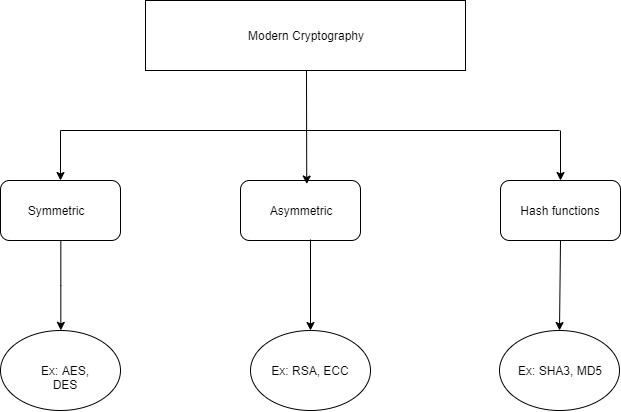
\includegraphics[width=14cm]{Thesis/images/types_of_cryptography.jpg}
    \caption{Types of Cryptography}
    \label{fig:figure21}
\end{figure*}


\newpage
\subsection{Symmetric Cryptography}

Here, a single key is used for both encryption and decryption. The sender uses a key to encrypt the plaintext and send ciphertext to the receiver, the receiver applies the same key which applied by send to decrypt the message and recover the plain text. In order to achieve this type of encryption both sender and receiver must share the common key via a secure medium or in person to avoid the revelation of the public key. Advanced Encryption Standard (AES), and Data Encryption Standard (DES) are good examples of Symmetric key Cryptography.

\subsection{Asymmetric Cryptography}

In this type of Cryptography, there are two keys are used, Public key and Private key. Public key can be shared between sender and receiver for encryption. But the private key remains secret for decryption. This type of decryption is more secure than the symmetric type. Even though the public key is shared, and it can be accessed to eaves dropper, he can’t easily find the secret key until he has the quantum computer with greater power. The most commonly used algorithms are RSA (RSA stands for Ron Rivest, Adi Shamir and Leonard Adleman) and ECC (Elliptic Curve Cryptography).

\subsection{Hash Functions}
Hash functions are called One-way Encryption, since it cannot be reversed. It is different from Symmetric and Asymmetric key cryptography because it doesn’t use any keys. In Simple terms, hashing means taking an input string of any arbitrary length and giving out an output of fixed length. A good hash function also should not produce the same hash value from two different inputs. If it does, this is known as a collision. But usually, the hash functions are designed to be collision resistant, meaning that there is a very low probability that the same string would be created for different data. SHA1, SHA2 and SHA3 (Secure Hash Algorithms) and MD5 are the good examples of Hash functions.

\subsection{Quantum Cryptography}

In addition to these, Quantum Cryptography is one more type, which uses Quantum Phenomena to increase the protection over the data transferred between sender and receiver. One-time pad is the best example of Quantum Cryptography which is also called Quantum Key Distribution. Unless the eaves dropper disturbs the message, the message transferred remains unchanged. Once the eaves dropper tries to access the data, then the data become changed since its works on the uncertainty principle of Heisenberg. 

\section{Post Quantum Cryptography and NIST}
This is the most important topic of today’s world and I am going to concentrate on this topic for the research. The difference between Quantum cryptography and PQC is, Quantum cryptography is defined by Quantum mechanics principles instead of Classical principles. Where as PQC is public key cryptography and it is safe against the Quantum computer’s mathematical power. That’s why it’s also called Quantum resist or Quantum proof algorithms. National Institute of Standards and Technology has provided the platform in their website for cryptographers and mathematicians to come up with their own Quantum resist algorithms \cite{nist}. Below algorithms are finalized in round 2. 

\newpage
\subsection{Algorithms selected for ROUND 2 submissions}
1.	Bike \\
2.	Classic McEliece \\
3.	CRYSTALS-KYBER \\
4.	FrodoKEM \\
5.	HQC \\
6.	LAC \\
7.	LEDAcrypt \\
8.	NewHope \\
9.	NTRU \\
10.	NTRU prime \\
11.	NTS-KEM \\
12.	Rollo \\
13.	Round 5 \\
14.	RQC \\
15.	SABER \\ 
16.	SIKE \\
17.	Three Bears \\


\newpage

\chapter{Hardware Implementation of RSA using FPGA}

\section{Introduction}
%
In this digital era, cryptography plays a critical role in everyone’s daily life. We use a wide range of electronic devices and applications to help us with our everyday routine. Data stored and transmitted between two entities needs to be done in a secure manner to prevent them from reaching untrusted sources. Cryptography is a process followed to convert original message into ciphertext as part of encryption and convert the ciphertext back to original message in decryption.

Symmetric and asymmetric cryptography are two ways to secure original message from attackers. Symmetric cryptography uses same key to encrypt and decrypt and is therefore faster than asymmetric algorithms but isn’t secure enough. On the other
hand, to ensure higher security, asymmetric cryptography uses a public key to encrypt the message and private key to decrypt it. RSA and Elliptic Curve Cryptography (ECC) are some of the examples of asymmetric cryptography.

This chapter will focus on explaining the architecture of RSA and its implementation using efficient multiplication and exponentiation components on FPGA.

Related work, Theoretical concepts of RSA algorithm, Required components like Montgomery multiplication, Montgomery exponentiation, primality tests and its simulation results are explained in the following sections.

\section{Related Work}

There are multiple ways to perform RSA algorithms in efficient manner. For example, Dr. S. Nirmala \cite{nirmala:praveena} presented bypass multiplier technique for implementing modular units in RSA algorithm, which avoids unnecessary modulo multiplication and reduces register requirements for multiplier architecture.
Xinkai Yan \cite{yan:wu:zheng:xie} implemented hybrid Montgomery modular multiplier which uses Karatsuba and Knuth multiplication algorithms in different levels to implement large integer multiplication. Mostafizur Rahman \cite{rahman:rokon} presented RSA algorithm using interleaved modular multiplication technique and Square and multiply technique for exponentiation.

%
\section{RSA Algorithm}
%
RSA is a widely-used, highly secure public key cryptographic algorithm. It generates a public key with which user’s message is encrypted and a private key is generated to decrypt the message. Implementation of RSA is computationally expensive as it operates on large numbers.

Exponentiation operation is fundamental in RSA cryptosystems and it was a challenging task to implement the necessary blocks using efficient algorithms. These operations require high computations when implemented by software. To achieve high security and greater performance, it is often more advantageous to design and develop cryptosystems in hardware \cite{mario:guillermo:francisco}.

\begin{figure*}[htp]
    \centering
    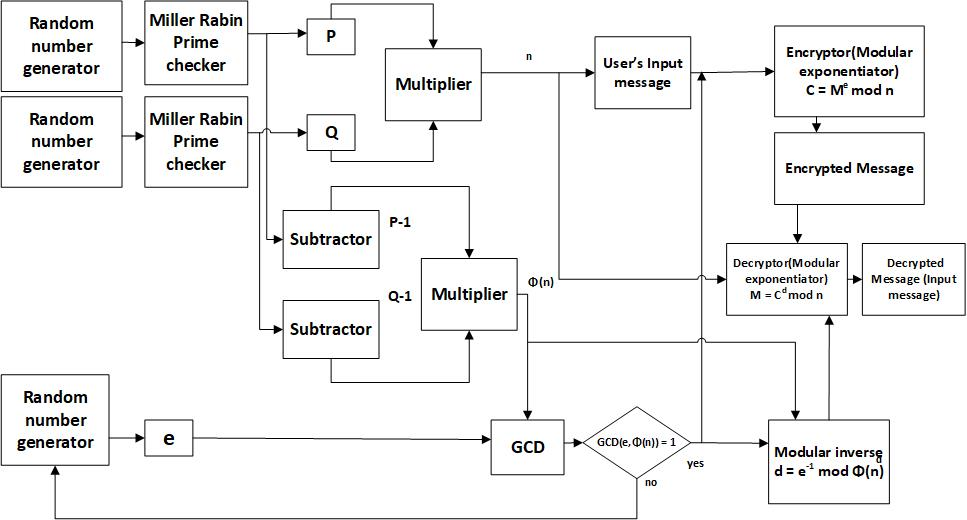
\includegraphics[width=14cm]{Thesis/images/RSA_Block_Diagram.jpg}
    \caption{Block diagram of RSA algorithm}
    \label{fig:figure1}
\end{figure*}

\newpage

Fig. \ref{fig:figure1} explains the complete block diagram of RSA algorithm. It starts with generating two large random prime numbers $p$, $q$ and $n$ is computed by multiplying the prime numbers using add-and-shift multiplier.

\begin{equation}
\label{eq1}
n = p \times q
\end{equation}

$\phi(n)$ is computed by multiplying the outputs of subtractor of prime numbers $p$ and $q$

\begin{equation}
\label{eq2}
\phi(n) = (p - 1) \times (q - 1)
\end{equation}

A random number $e$ is generated such that it is between 1 and $\phi(n) - 1$, and the Greatest Common Divisor (GCD) of $e$ and $\phi(n)$ is 1. A random number generator block and GCD block generates this public key in hardware.

\begin{equation}
\label{eq3}
e \in \{1,2,3...\phi(n) - 1\}, GCD(e, \phi(n)) = 1
\end{equation}

The following public key is used to encrypt the incoming message to obtain cipher-text

\begin{equation}
\label{eq4}
C = M^e\,mod\,n
\end{equation}

A private key $d$ is generated using modular inverse operation from $e$ and $\phi(n)$ by

\begin{equation}
\label{eq5}
d = e^{-1}\,mod\,\phi(n)
\end{equation}

Using the above generated private key, the original message can be decrypted back from the cipher-text by

\begin{equation}
\label{eq6}
M = C^d\,mod\,n
\end{equation}

Figure \ref{fig:figure2} and Figure \ref{fig:figure3} shows power estimation and utilization summary of RSA respectively. Figure \ref{fig:figure4} shows simulation results of the RSA algorithm designed and implemented using Very High-Speed Integrated Circuit Hardware Description Language (VHDL) on Xilinx Vivado Design Suite. Random prime numbers $p$ and $q$ are represented as $reg \text{\textunderscore} p$ and $reg \text{\textunderscore} q$ respectively in the program, and their product is stored as $reg \text{\textunderscore} n$. Input $message$ is encrypted into $cipher \text{\textunderscore} text$ using public key $reg \text{\textunderscore} n$ and $reg \text{\textunderscore} e$. $cipher \text{\textunderscore} text$ is then decrypted back to input message using private key $reg \text{\textunderscore} d$.

\newpage

\begin{figure}[htp]
    \centering
    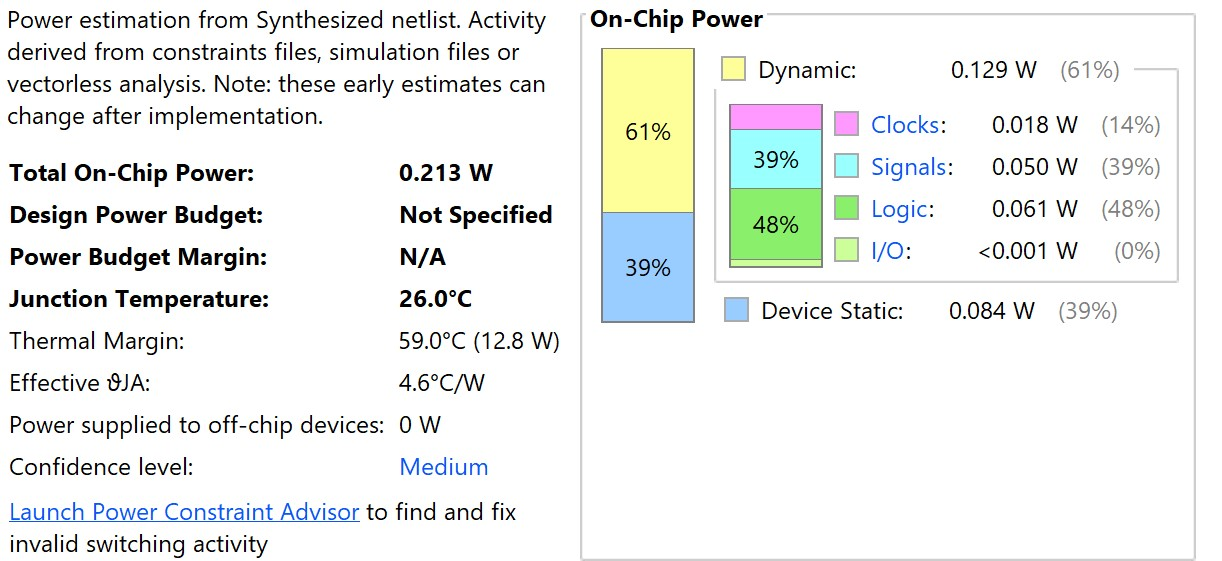
\includegraphics[width=14cm]{Thesis/images/RSA_Power_Estimation.jpg}
    \caption{Summary of power estimation for 16-bit RSA}
    \label{fig:figure2}
\end{figure}

\begin{figure}[htp]
    \centering
    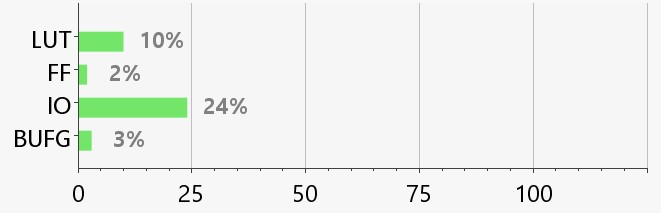
\includegraphics[width=14cm]{Thesis/images/RSA_Utilization_Summary.jpg}
    \caption{Utilization summary for RSA}
    \label{fig:figure3}
\end{figure}

\newpage

\begin{figure*}[htp]
    \centering
    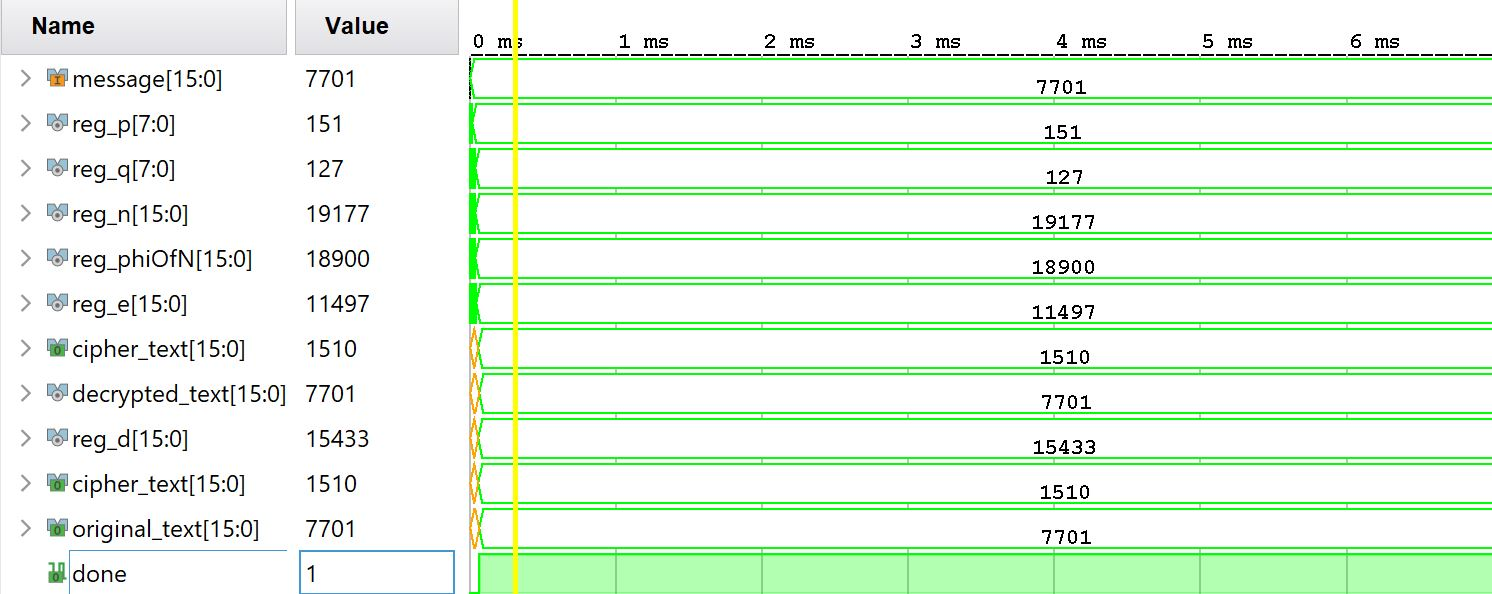
\includegraphics[width=14cm,height=6cm]{Thesis/images/RSA_Simulation_Results.jpg}
    \caption{Simulation results of encryption and decryption blocks of RSA}
    \label{fig:figure4}
\end{figure*}

Since this implementation is utilizing 10\% of look-up tables, 10 similar blocks can be implemented on a Nexys4 FPGA board.

\subsection{Montgomery Multiplication}

Multiplication and division require complex computations when implemented in hardware platforms. In a traditional approach, modular multiplication involves multiplication followed by division \cite{hans:nils:sheueling:vipul:leonard}. Equation \eqref{eq4} and \eqref{eq6} shows the need to compute modular exponentiation in RSA, each requiring lots of modular multiplication components. There are many approaches to perform multiplication such as multiply then divide, interleaving multiplication and reduction, Brickell's method \cite{sushanta:manoranjan}.

\newpage

\begin{figure}[H]
    \centering
    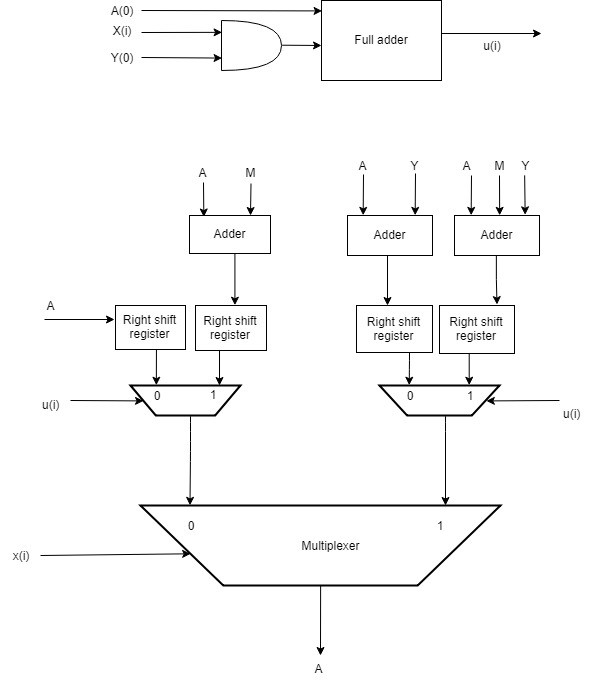
\includegraphics[width=14cm]{Thesis/images/Modular_Multiplier_Architecture.jpg}
    \caption{Architecture of Montgomery modular multiplier}
    \label{fig:figure5}
\end{figure}

\newpage

To design and develop an efficient crypto-processor, Montgomery multiplication  has been chosen for all our modular multiplication calculations. This technique avoids the traditional division operation, and replaces it with shift-and-add operation. Montgomery modular multiplication is computed as

\begin{equation}
\label{eq7}
\centering
\begin{aligned}
  A = X \times Y \times R^{-1}\,mod\,M\\
  &\\
  R = 2^n, \textrm{where $n$ is number of bits}  
\end{aligned}
\end{equation}

Equation \eqref{eq7} represents a modular multiplication in Montgomery domain. Results of the above computation can remain in Montgomery domain, as converting it back to real world coordinates is a costly operation. Since we use Montgomery exponentiation, it can handle the results of modular multiplication in Montgomery domain and avoids the need to convert it back \cite{manish:amit:aakanksha:abhinav}.

Two preconditions for Montgomery multiplication technique are 

\begin{itemize}

\item Modulus $M$ needs to be co-prime with $R$\\
i.e. $GCD (M, R) = 1$

\item Multiplicand and multiplier need to be smaller than modulus $M$ \cite{nadia:luiza}

\end{itemize}

Montgomery multiplier requires $2n(n+1)$ single-precision multiplications due to $n$ loop iterations as seen in Algorithm \ref{algorithm1}. As the result is computed in Montgomery domain, converting it back to real world coordinates requires additional single-precision operations, thereby having a total of $4n(n+1)$ single-precision multiplications. This is slower than the traditional multiplication algorithms, which perform at $2n (n+1)$ computational efficiency. Since we don't convert it to real world coordinates and the results of multiplication can be used in exponentiation component in Montgomery domain, this is an efficient modular multiplication technique \cite{alfred:paul:scott}.

\begin{algorithm}
\caption{Montgomery modular multiplication algorithm \cite{alfred:paul:scott}}\label{multiply}
\begin{algorithmic}[1]
\State \text{Inputs: } $X, Y, M$
\State \text{Ouput: } $A = XYR^{-1} mod M$
\State $\textit{A} \gets \text{zeros for }\textit{n + 1}$ bits
\State $b = 2$
\State $M' = M^{-1} mod b$
\For {i: from 0 to n - 1} 
    \State $u(i) = (A_{0} + X_{i} \times Y_{0}) \times M' mod b$ 
    \State $A = \frac{A + X_{i} \times Y + u(i) \times M}{2}$
\EndFor
\If {$A >= M$}
    \State $A = A - M$
\EndIf
\State Return A
\end{algorithmic}
\label{algorithm1}
\end{algorithm}

\begin{table}[h]
\centering
\caption{Utilization summary of Montgomery multiplication}
\begin{tabular}{llll}
\hline
Resource &
Utilization &
Available &
Utilization \% \\
\hline
LUT &
48 &
63400 &
0.08 \\
FF &
29 &
126800 &
0.02 \\
IO &
19 &
210 &
9.05 \\
BUFG &
1 &
12 &
3.13 \\
\hline
\end{tabular}
\label{table:table1}
\end{table}

\begin{figure}[htp]
    \centering
    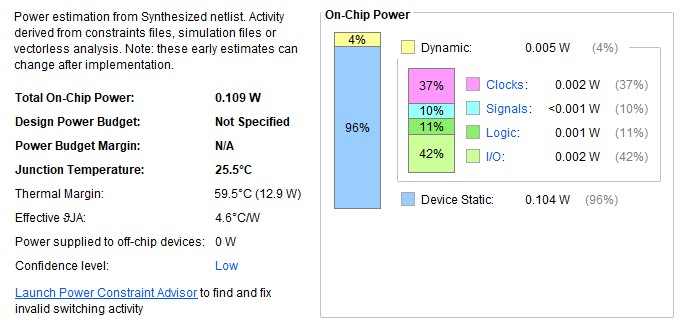
\includegraphics[width=14cm]{Thesis/images/Montgomery_Multiplier_Power_Estimation.jpg}
    \caption{Summary of power estimation for 16-bit Montgomery multiplier}
    \label{fig:figure6}
\end{figure}

For every iteration $i$ in the algorithm, $u(i)$ is computed using a Full Adder, and the divide operation is performed using a right-shift register as shown in the architecture in the Figure \ref{fig:figure5}. The entire algorithm is designed and implemented using Xilinx Vivado Design Suite. Figure \ref{fig:figure7} shows the simulation results of 16-bit Montgomery multiplication.

\begin{figure*}[htp]
    \centering
    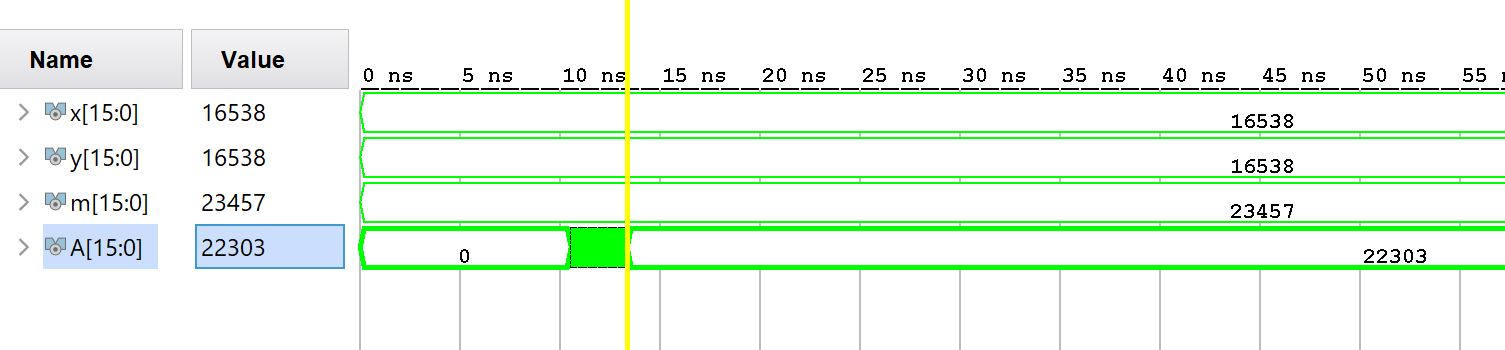
\includegraphics[width=14cm, height=4cm]{Thesis/images/Modular_Multiplier_Simulation_Results.jpg}
    \caption{Simulation results of Montgomery multiplier from Xilinx Vivado Design Suite}
    \label{fig:figure7}
\end{figure*}

Very High-Speed Integrated Circuit Hardware Description Language (VHDL) is the language used to describe the hardware design. A test bench has been written to verify the design for variable bit sizes. The program has been then synthesized and implemented on a Nexys4 FPGA board. Table \ref{table:table1} shows the utilization summary on implementing the algorithm on FPGA board.

\newpage

\subsection{Montgomery Exponentiation}

\begin{figure}[htp]
    \centering
    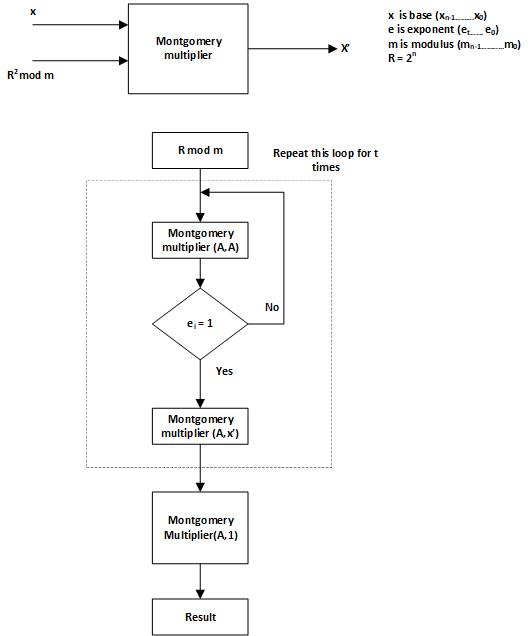
\includegraphics[width=14cm, height=12cm]{Thesis/images/Montgomery_Exponentiation_Flowchart.jpg}
    \caption{Flowchart for Montgomery Exponentiation}
    \label{fig:figure8}
\end{figure}

Figure \ref{fig:figure8} shows the architecture of Montgomery exponentiation. It involves 4 Montgomery multiplier blocks and is repeated over $t$ iterations, where $t$ is number of bits in the exponent.

\begin{equation}
\label{eq8}
Result (A) = x^e\,mod\,m
\end{equation}

As the entire algorithm is carried out using Montgomery multiplication, result remain in Montgomery domain and the final step of equation \eqref{eq9} converts it to real world coordinates.

\begin{equation}
\label{eq9}
A = Mont(A, 1)
\end{equation}

Figure \ref{fig:figure9} shows the simulation results of Montgomery exponentiation component for 16 bits using Xilinx Vivado Design Suite. Since each block of RSA algorithm was designed and developed as a stand-alone reusable component, they can be simulated to verify the design, synthesized and implemented on FPGA board. Montgomery exponentiation utilizes $~3\%$ of look-up tables on Nexys4 FPGA board as seen in Table \ref{table:table2}.

\begin{table}[h]
\centering
\caption{Utilization summary of Montgomery exponentiation algorithm}
\begin{tabular}{llll}
\hline
Resource &
Utilization &
Available &
Utilization \% \\
\hline
LUT &
1796 &
63400 &
2.83 \\
FF &
2696 &
126800 &
2.13 \\
IO &
18 &
210 &
8.57 \\
BUFG &
2 &
32 &
6.25 \\
\hline
\end{tabular}
\label{table:table2}
\end{table}

\begin{figure*}[htp]
    \centering
    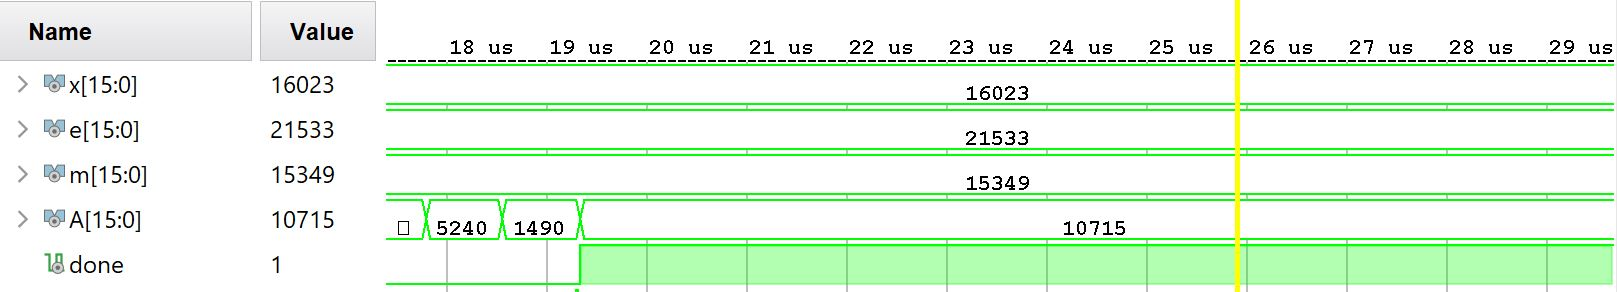
\includegraphics[width=14cm, height=4cm]{Thesis/images/Montgomery_Exponentiation_Simulation_Results.jpg}
    \caption{Simulation results of Montgomery exponentiation}
    \label{fig:figure9}
\end{figure*}

\subsection{Miller Rabin Primality Test}
Primality tests are computationally expensive since it involves repeated exponentiation and modular multiplications. RSA algorithm begins with the need to generate two random prime numbers. Random numbers were generated on FPGA using Linear Feedback Shift Register (LFSR). These random numbers were passed onto a primality test before they can be used further in the algorithm. We chose Miller Rabin to confirm primality of random numbers. This is mainly due to the ability to configure witness count parameter in the algorithm. The higher the witness count, higher the number of iterations to generate a strong prime number. Another advantage of Miller Rabin is the way it breaks the loop as soon as it finds a composite number as shown in Figure \ref{fig:figure10}.

Error probability of Miller Rabin is less than $(1/4)^t$, where $t$ is witness count. This algorithm has also proven to be better than Fermet's primality test and Solovay-Strassen test due to the computational costs involved in calculating modular multiplications \cite{alfred:paul:scott}. Figure \ref{fig:figure10} shows the usage of a reusable random number generator block and modular exponentiation block in Miller Rabin primality tester algorithm.

\newpage
\begin{figure*}[htp]
    \centering
    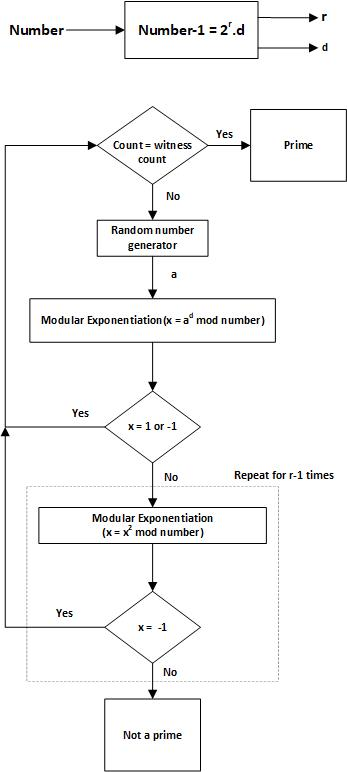
\includegraphics[width=8cm]{Thesis/images/Miller_Rabin_Primality_Test_Architecture.jpg}
    \caption{Architecture of Miller Rabin Primality Test}
    \label{fig:figure10}
\end{figure*}




\newpage
\section{Use case: Monitoring of cyberphysical systems}
Devoloped RSA cryptoprocessor can be beneficial for IoT systems.
IoT requiring strong security as well as low resource consumption
is emerging in many different domains, particularly
related to critical applications where data integrity, confidentiality
and privacy are of paramount importance. IoT with
secure wireless communication is required for the protection
of cyber-physical systems with limited wiring possibilities,
such as industry production chains with moving parts. Digital
Twins (DT) in the Industrial IoT are an example of them. A
DT is a digital model of a production system elaborated in
conjunction with a digital model of the product generated, and
paves the way to Collaborative Manufacturing, with strong
enhancements for distributed quality control and information
sharing. In those scenarios, sensing technologies can be deployed
to create an interconnected system of systems, where
data collection points can be leveraged to provide real-time
and high-accuracy monitoring of cyber-physical models, prevent
quality degradation and keep track of deviations from
production specifications. Production systems, e.g., CNC and
robots, can communicate with the supervisory software to
keep track of the production operations, and along with the
sensors installed on the products (e.g., car components) to
determine the current state of the physical parameters. Bluetooth
modules can be mounted on reconfigurable electronics
equipped with physical sensors devoted to the monitoring of
cyber-physical parameters of Digital Twins. This hardware implementation of RSA has following features:

• FPGA resources can be significantly saved, in particular
power consumption

• Remaining FPGA electronics can be devoted to model
tracking and edge intelligence in the cyber-physical
systems (e.g., a Digital Twin)

• Encryption modules can be made stronger using many
reconfigurable low-power crypto-modules

• Scalability and accuracy of cyber-physical models can
improve due to the possibility to upload more often due
to low energy consumption

\section{Evaluation}
In terms of turnout time, Mostafizur Rahman’s square and
multiply technique \cite{rahman:rokon} took 95$\mu$s to complete the exponentiation
operation, but proposed Montgomery technique took only
19$\mu$s to complete the exponentiation. In terms of power,
Prasanth kumar’s clock cycle method \cite{kumar:kumar:parthibane} for exponentiation
(32-bit) consumed 1.760 watt, power consumption using proposed
Montgomery technique for exponentiation (32-bit) is 0.424
watt.

\chapter{Quantum Implementation of RSA using Qiskit}
\section{Difference between classical computers and Quantum computers}
Classical computers are computers we use every day for all the tasks, and they work based on bits (0’s and 1’s). We can imagine a bit as a switch which has only two states, ON and OFF. But Quantum computers on the other hand uses a special bit called Qubit. We can imagine a qubit as a sphere. On the surface of the sphere, if the qubit faces up then it’s called $|$0$>$ state, if it faces down, then it’s called $|$1$>$ state. Those states are equivalent to ordinary bit state 0 and 1 respectively. But Qubit has another state on the sphere’s surface which is the value between and $|$0$>$ and $|$1$>$, meaning $|$0$>$ and $|$1$>$ at the same time, called superposition state. In figure \ref{fig:figure11}, superposition state is denoted as u3(0.5*pi,0,0) $|$0$>$. The value of the qubit can’t be directly outputted. And it must be measured and stored in classical bits before any read and write operation.

\begin{figure*}[htp]
    \centering
    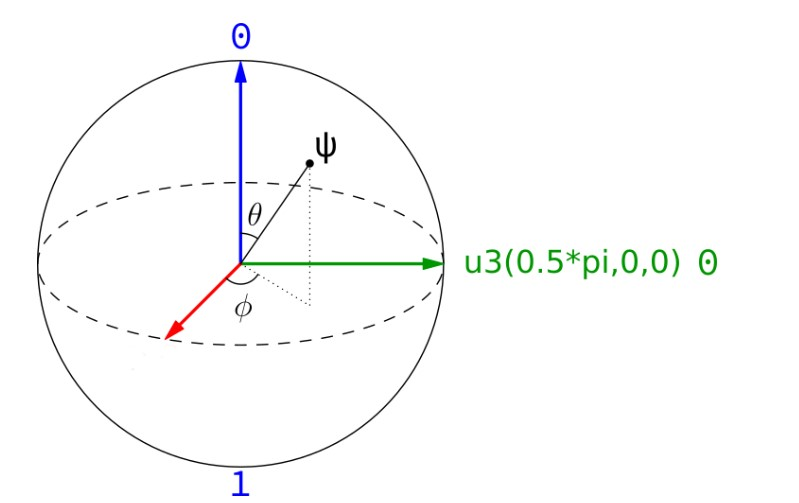
\includegraphics[width=8cm]{Thesis/images/Block_sphere_for_qubit_representation.jpg}
    \caption{Block sphere for qubit representation}
    \label{fig:figure11}
\end{figure*}

In classical computers, if we use two bits, then we can represent four states. But we can represent only one state at a time. Hence, number of calculations takes time. Especially in cryptography, this limitation allows us to achieve the security level we need. For example, the secure property of RSA relies on the factorization problem. Multiplying two prime numbers are easy to calculate. But getting back the prime numbers from having the product is difficult. It takes millions of years to calculate in classical computers, since only one state can be re-presentable at a time.  While in Quantum computers, if we use n qubits, we can represent 2$^n$ states simultaneously \cite{quantum_computing_medium}. Adding one qubit to the system, increases its power exponentially. 
\section{Introduction to Qiskit}

Qiskit is an open source SDK (Software Development Kit) created by IBM, which allows us to access real Quantum computer via cloud. % reference [https://arxiv.org/pdf/1903.04359.pdf]%. 
Before starting to code for Quantum computers, first we need to create an account with IBM Q experience to interact with Quantum simulator. A token will be generated for our account to access IBM’s Quantum computer \cite{sashwat_simple_adder}. Programs were written in Python in Jupyter Notebook to work with IBM's Quantum computer.

After installing Qiskit using \texttt{ pip install } command, first step to start coding in the IBM’s Quantum computer is to enable your account with the token provided in the IBM Q experience. This can be done by the following lines of code in Jupyter notebook.

\begin{lstlisting}[language=Python]
from qiskit import IBMQ
provider = IBMQ.enable_account('<your-token>')
qasm_sim = provider.get_backend('ibmq_qasm_simulator')
\end{lstlisting}

\section{Basic Quantum gates}
When we execute any program in classical computers, it converts the instructions into sequence of operations called logic gates. The same rule applies for Quantum computers as well. The only difference is, we do have completely different sets of gates for Quantum computers with very rare similarities. Here are some basic gates used in Quantum computers \cite{quantum_gates_book_ibm}. 

$X$ gate: It acts like a classical NOT, flipping a qubit $|$0$>$ state to $|$1$>$  state and $|$1$>$  state to $|$0$>$ state. This operation requires only one qubit. 

$CX$ gate (Controlled-X gate): This gate requires two qubits. One is called target qubit, and another is called control qubit. This gate applies an X gate to the target qubit only if control qubit is in the $|$1$>$ state.

\newpage
$CCX$ gate (Controlled-Controlled-X gate): This gate acts on three qubits. Two qubits act as control qubits and one qubit acts as target qubit. This gate applies X gate to the target qubit, if only both control qubits are in the $|$1$>$ state.


\section{Simple 7-bit Adder}

Step 1: Import

Import necessary modules from Qiskit and Python. Quantum registers are needed to store and perform the calculation on our inputs. Qubits from quantum registers can't be printed directly in classical computers, hence they will be measured and stored in classical registers. Import \texttt{ ClassicalRegister } and \texttt{ QuantumRegister } from Qiskit. Quantum circuit is needed to form a circuit in Quantum hardware. \texttt{ execute } module needs to be imported from Qiskit to execute a quantum circuit \cite{sashwat_simple_adder}. 

Once all the necessary modules are imported as below, enable your account if its not already enabled. 

\begin{lstlisting}[language=Python]
from qiskit import ClassicalRegister, QuantumRegister
from qiskit import QuantumCircuit
from qiskit import execute
from qiskit import IBMQ

provider = IBMQ.enable_account('<your-token>')
qasm_sim = provider.get_backend('ibmq_qasm_simulator')
\end{lstlisting}

\newpage
Step 2: Get user input

Get two input numbers from user in the form of bits as shown in below code snippet. If the length of the first number is greater than the second number, then assign the first number length’s to sum’s length else do the opposite. 

\begin{lstlisting}[language=Python]
first = input("Enter a binary number with less than 8 digits")
second = input("Enter another number with less than 8 digits")

l = len(first)
l2 = len(second)
if l > l2:
     n = l
else:
     n = l2
\end{lstlisting}

Step 3: Initializing registers

\begin{lstlisting}[language=Python]
#Initializing the registers; two quantum registers with n bits each
#1 more with n+1 bits, which will also hold the sum of the two #numbers
#The classical register has n+1 bits, which is used to make the sum #readable
a = QuantumRegister(n) #First number
b = QuantumRegister(n+1) #Second number, then sum
c = QuantumRegister(n) #Carry bits
cl = ClassicalRegister(n+1) #Classical output
#Combining all of them into one quantum circuit
qc = QuantumCircuit(a, b, c, cl)
\end{lstlisting}

\newpage
Step 4: Loading the input to Quantum registers using $X$ gate

When quantum registers are initialized, by default every qubit is in $|$0$>$ state. If we want to load appropriate value, we need to check bit by bit and apply $X$ gate where $|$1$>$ should be placed. 

\begin{lstlisting}[language=Python]
#Setting up the registers using the values inputted
for i in range(l):
    if first[i] == "1":
        qc.x(a[l - (i+1)]) #Flip the qubit from 0 to 1
for i in range(l2):
    if second[i] == "1":
        qc.x(b[l2 - (i+1)]) #Flip the qubit from 0 to 1
\end{lstlisting}

Quantum registers $a$ and $b$ hold the value of two numbers to be added. 

Step 5: Calculate carry output and sum output

\begin{table}[h]
\centering
\caption{Truth table to calculate carry output}
\begin{tabular}{llll}
\hline
$C$ &
$A$ &
$B$ &
$C_{i+1}$ \\
\hline
0 &
0 &
0 &
0 \\
0 &
0 &
1 &
0 \\
0 &
1 &
0 &
0 \\
0 &
1 &
1 &
1 \\
1 &
0 &
0 &
0 \\
1 &
0 &
1 &
1 \\
1 &
1 &
0 &
1 \\
1 &
1 &
1 &
1 \\
\hline
\end{tabular}
\label{table:table3}
\end{table}

\newpage
\begin{figure*}[htp]
    \centering
    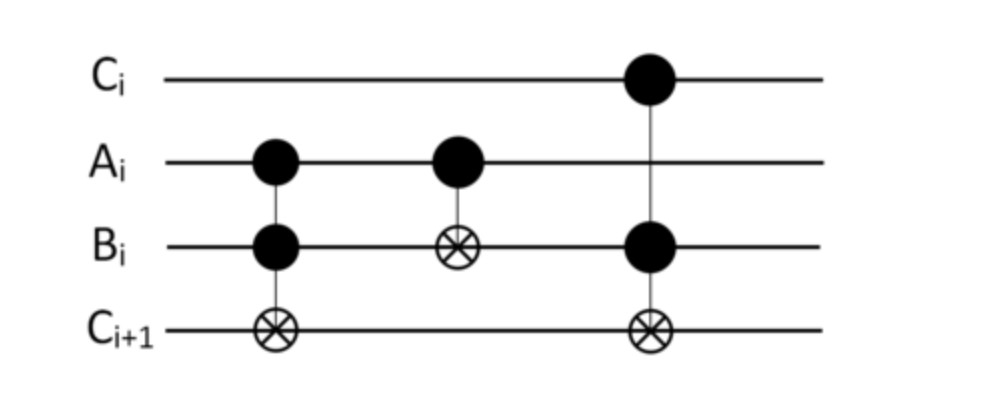
\includegraphics[width=14cm]{Thesis/images/Quantum_carry_output_circuit.jpg}
    \caption{Quantum circuit for carry output}
    \label{fig:figure17}
\end{figure*}

The lines with two filled in circles and one hollowed out circle with a cross represent the $CCX$ gates, and the one with one of each circle represents the $CX$ gate. Below code processes $n-2$ bits.

\begin{lstlisting}[language=Python]
#Implementing a carry gate that is applied on all 
#(c[i], a[i], b[i]) #with output fed to c[i+1]
for i in range(n-1):
    qc.ccx(a[i], b[i], c[i+1])
    qc.cx(a[i], b[i])
    qc.ccx(c[i], b[i], c[i+1])
\end{lstlisting}

Since $b$ register is used to store the sum of $a$ and $b$, instead of creating an extra carry bit for the last carry, and then transferring that to register $b$, we can substitute the last qubit of $b$ for the last carry bit.

\newpage
\begin{lstlisting}[language=Python]
#For the last iteration of the carry gate, 
#instead of feeding the #result to c[n], 
#we use b[n], which is why c has only n bits, 
#with #c[n-1] being the last carry bit
qc.ccx(a[n-1], b[n-1], b[n])
qc.cx(a[n-1], b[n-1])
qc.ccx(c[n-1], b[n-1], b[n])
\end{lstlisting}

Carry outputs are all stored in $c[i+1]$ and extra bit $b[n]$. Operation performed on input qubits needs to be reversed. Reversing is an easy operation, since all the Quantum logic gates are reversible by applying the same gate on the inputs. This is done to make sure the correct inputs are fed to calculate the sum output.

Sum can easily be calculated in classical computers using boolean logic gates. Challenge has been to find a quantum equivalent to perform the same operation. To calculate sum, a gate that can take three input qubits is needed: input carry qubit, and one qubit from each of the addends. The gate would perform an operation that would achieve the same results as shown in table \ref{table:table4}

\newpage
\begin{table}[h]
\centering
\caption{Truth table to calculate sum}
\begin{tabular}{llll}
\hline
$C$ &
$A$ &
$B$ &
$Sum$ \\
\hline
0 &
0 &
0 &
0 \\
0 &
0 &
1 &
1 \\
0 &
1 &
0 &
1 \\
0 &
1 &
1 &
0 \\
1 &
0 &
0 &
1 \\
1 &
0 &
1 &
0 \\
1 &
1 &
0 &
0 \\
1 &
1 &
1 &
1 \\
\hline
\end{tabular}
\label{table:table4}
\end{table}

Result couldn't be achieved by using one quantum gate, hence, multiple quantum gates will be combined as explained below:

1.	Apply $CX$ gate to $C$ (Carry in) and $B$ qubits where $C$ is the control qubit and $B$ is the target qubit. When $C$ is in $|$1$>$ state, flip the $B$ qubit. 
2.	Apply $CX$ gate to $A$ and $B$ qubits where $A$ is the control qubit and $B$ is the target qubit. When A is in $|$1$>$ state, flip the $B$ qubit. 
3.	Store the sum results in $B$ qubit. 

These steps are represented as a Quantum circuit as shown in figure \ref{fig:figure18}

\begin{figure*}[htp]
    \centering
    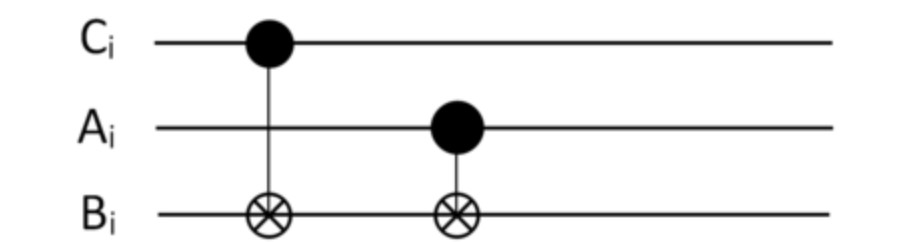
\includegraphics[width=14cm]{Thesis/images/Quantum_sum_output_circuit.jpg}
    \caption{Quantum circuit for sum output}
    \label{fig:figure18}
\end{figure*}

The line with one dark circle and one crossed circle represents $CX$ gate.

\begin{lstlisting}[language=Python]
#Reversing the gate operation performed on b[n-1]
qc.cx(c[n-1], b[n-1])
#Reversing the gate operations performed 
#during the carry gate implementations
#This is done to ensure the sum gates are fed 
#with the correct input bit states
for i in range(n-1):
    qc.ccx(c[(n-2)-i], b[(n-2)-i], c[(n-1)-i])
    qc.cx(a[(n-2)-i], b[(n-2)-i])
    qc.ccx(a[(n-2)-i], b[(n-2)-i], c[(n-1)-i])
    #These two operations act as a sum gate; if a control bit is at                
    #the 1> state then the target bit b[(n-2)-i] is flipped
    qc.cx(c[(n-2)-i], b[(n-2)-i])
    qc.cx(a[(n-2)-i], b[(n-2)-i])
\end{lstlisting}

Step 6: Measure qubits and store the results in classical registers

Since qubits can't be extracted for any useful information, they will be measured and stored in classical registers.

\begin{lstlisting}[language=Python]
#Measure qubits and store results in classical register cl
for i in range(n+1):
    qc.measure(b[i], cl[i])
\end{lstlisting}

\newpage
Step 7: Execute job in IBMQ simulator

\begin{lstlisting}[language=Python]
#Set chosen backend and execute job
num_shots = 2 #Setting the number of times to repeat measurement
job = execute(qc, qasm_sim, shots=num_shots)
#Get results of program
job_stats = job.result().get_counts()
print(job_stats)
\end{lstlisting}

\section{Quantum Fourier Transform based Adder}

Previous implementation of n-bit addrer shows a classical approach to solve the problem using Qiskit. To achieve fast addition, quantum-ness of qubits needs to be taken into account while programming the adder circuit. This section explains the implementation of fast adder using Quantum Fourier Transform \cite{sashwat_fast_adder}.

In 2019 IBM is set to release its biggest quantum computer consisting of 53 qubits. However, at the time of this research, only 32 qubits quantum computer are available for public use, which can be used to add maximum 9 qubits because, $n+1$ qubits is needed to store each inputs and another $n+1$ qubits to store the output. A total of $3n+3$ qubits are needed for quantum addition operation. 

\newpage
Step 1: Import modules and get user input

If user inputs are of different length, pad zeros to make it convinient to apply Quantum Fourier Transform (QFT)

\begin{lstlisting}[language=Python]
from QFTAddition import add
from qiskit import ClassicalRegister, QuantumRegister
from qiskit import QuantumCircuit
from qiskit import execute
from qiskit import IBMQ
import math
import operator

provider = IBMQ.enable_account('<your-token>')
qasm_sim = provider.get_backend('ibmq_qasm_simulator')

#Take two numbers as user input in binary form   
first = input("Enter a number with less than 10 digits.")
second = input("Enter another number with less than 10 digits.")

l1 = len(first)
l2 = len(second)
#Making sure that 'first' and 'second' are of the same length 
#by padding the smaller string with zeros
if l2>l1:
    first,second = second, first
    l2, l1 = l1, l2
second = ("0")*(l1-l2) + second
\end{lstlisting}

\newpage
Step 2: Create separate functions for QFT operations

There are three functions for QFT addition procedure:

1.	CreateInputState()

2.	evolveQFTState()

3.	Inverse QFTState()

The first function CreateInputState() is used to convert the first number into QFT form by applying some of the quantum gates. Here are following rules to convert a number to QFT form.

•	Let $n$ be the length of first number.

•	Apply a Hadamard gate on the qubit in register $a$ with index $n$.

•	Starting from the index of the qubit passed, count backwards until you reach zero. Let’s call this number $m$.

•	Each time you count down once, apply a controlled rotation gate, controlled by the qubit in register $a$ with index $n$ on the qubit in register $a$ with index $m$.

•	This rotation gate would be called with parameter equal to $\frac{\pi}{2 ^ {n - m}}$

\begin{lstlisting}[language=Python]
def createInputState(qc, reg, n, pie):
    """
    Apply one Hadamard gate to the nth qubit of the quantum register               
    reg, and then apply repeated phase rotations with parameters  
    being pi divided by increasing powers of two.
    """
    qc.h(reg[n])    
    for i in range(0, n):
        qc.cu1(pie/float(2**(i+1)), reg[n-(i+1)], reg[n])
\end{lstlisting}

Next, evolveQFTstate() function is created to perform controlled rotations on the qubits of the register holding the first number, controlled by the qubits of the second number. Here are few rules for writing this function:

•	Let $n$ be the passed index.

•	Starting from the index of the qubit passed, count backwards until you hit -1, given by the number $m$. Before you count down once, apply a controlled rotation gate controlled by the qubit in register $b$ with index $m$ on the qubit in register $a$ with index $n$.

\begin{lstlisting}[escapeinside={(*}{*)}, language=Python]
def evolveQFTState(qc, reg_a, reg_b, n, pie, factor):
    """  
    Evolves the state |F((*$\psi$*)(reg_a))> to |F((*$\psi$*)(reg_a+reg_b))> using the   
    quantum Fourier transform conditioned on the qubits of the 
    reg_b. Apply repeated phase rotations with parameters being pi 
    divided by increasing powers of two.
    """
    l = len(reg_b)
    for i in range(0, n + 1):
        if (n - i) > l - 1:
            pass
        else:
            qc.cu1(factor * pie / float(2**(i)), reg_b[n - i], reg_a[n])
\end{lstlisting}

\newpage
inverseQFT() function would perform the same sequence performed in createInputState() function, but in reverse order. This would involve a new set of rules:

•	Let $n$ be the passed index.

•	Starting from -1, count up until you reach $n$. Let’s call the number you are at $m$.

•	Each time you count up once, apply a controlled rotation gate, controlled by the qubit in register $a$ with index $n$ on the qubit in register $a$ with index $n-m-1$.

•	Apply a Hadamard gate to the qubit in register $a$ with index $n$.

\begin{lstlisting}[language=Python]
def inverseQFT(qc, reg, n, pie):
    """
    Performs the inverse quantum Fourier transform on a register 
    reg. Apply repeated phase rotations with parameters being pi    
    divided by decreasing powers of two, and then apply a Hadamard 
    gate to the nth qubit of the register reg.
    """
    for i in range(0, n):
        qc.cu1(-1*pie/float(2**(n-i)), reg[i], reg[n])
    qc.h(reg[n])
\end{lstlisting}

Once all functions were defined, quantum circuits can be created to perform QFT based addition.

\newpage
Step 4: Creating Quantum registers, Classical Registers and Quantum circuit

\begin{lstlisting}[language=Python]
n = len(first)
pie = math.pi
a = QuantumRegister(n+1, "a") #Holds the first number
b = QuantumRegister(n+1, "b") #Holds the second number 
cl = ClassicalRegister(n+1, "cl") #Holds the final output
qc = QuantumCircuit(a, b, cl, name="qc")
\end{lstlisting}

Step 5: Loading the input to Quantum registers

\begin{lstlisting}[language=Python]
#Flip the corresponding qubit in register a if a bit in the 
#string first is a 1
for i in range(0, n):
    if first[i] == "1":
        qc.x(a[n-(i+1)])
#Flip the corresponding qubit in register b if a bit in the 
#string second is a 1
for i in range(0, n):
    if second[i] == "1":
        qc.x(b[n-(i+1)])
\end{lstlisting}

Step 6: Using QFT functions for addition operation

\begin{lstlisting}[escapeinside={(*}{*)}, language=Python]
# Compute the Fourier transform of register a
for i in range(0, n):
    createInputState(circ, reg_a, n - (i+1), pie)
# Add the two numbers by evolving the Fourier transform   
# F((*$\psi$*)(reg_a))> to |F((*$\psi$*)(reg_a+reg_b))>
for i in range(0, n):
    evolveQFTState(circ, reg_a, reg_b, n - (i+1), pie, factor)
# Compute the inverse Fourier transform of register a
for i in range(0, n):
    inverseQFT(circ, reg_a, i, pie)
\end{lstlisting}

Step 7: Executing the circuit in Quantum hardware using API token

\begin{lstlisting}[language=Python]
for i in range(0, n+1):
    qc.measure(a[i], cl[i])
    
#Select backend and execute job
result = execute(qc, backend= qasm_sim, shots=512).result()
counts = result.get_counts("qc")
print(counts)
\end{lstlisting}

Quantum circuit of QFT adder is shown in figure\ref{fig:figure12}, figure \ref{fig:figure13} and figure \ref{fig:figure14}.

\begin{figure*}[htp]
    \centering
    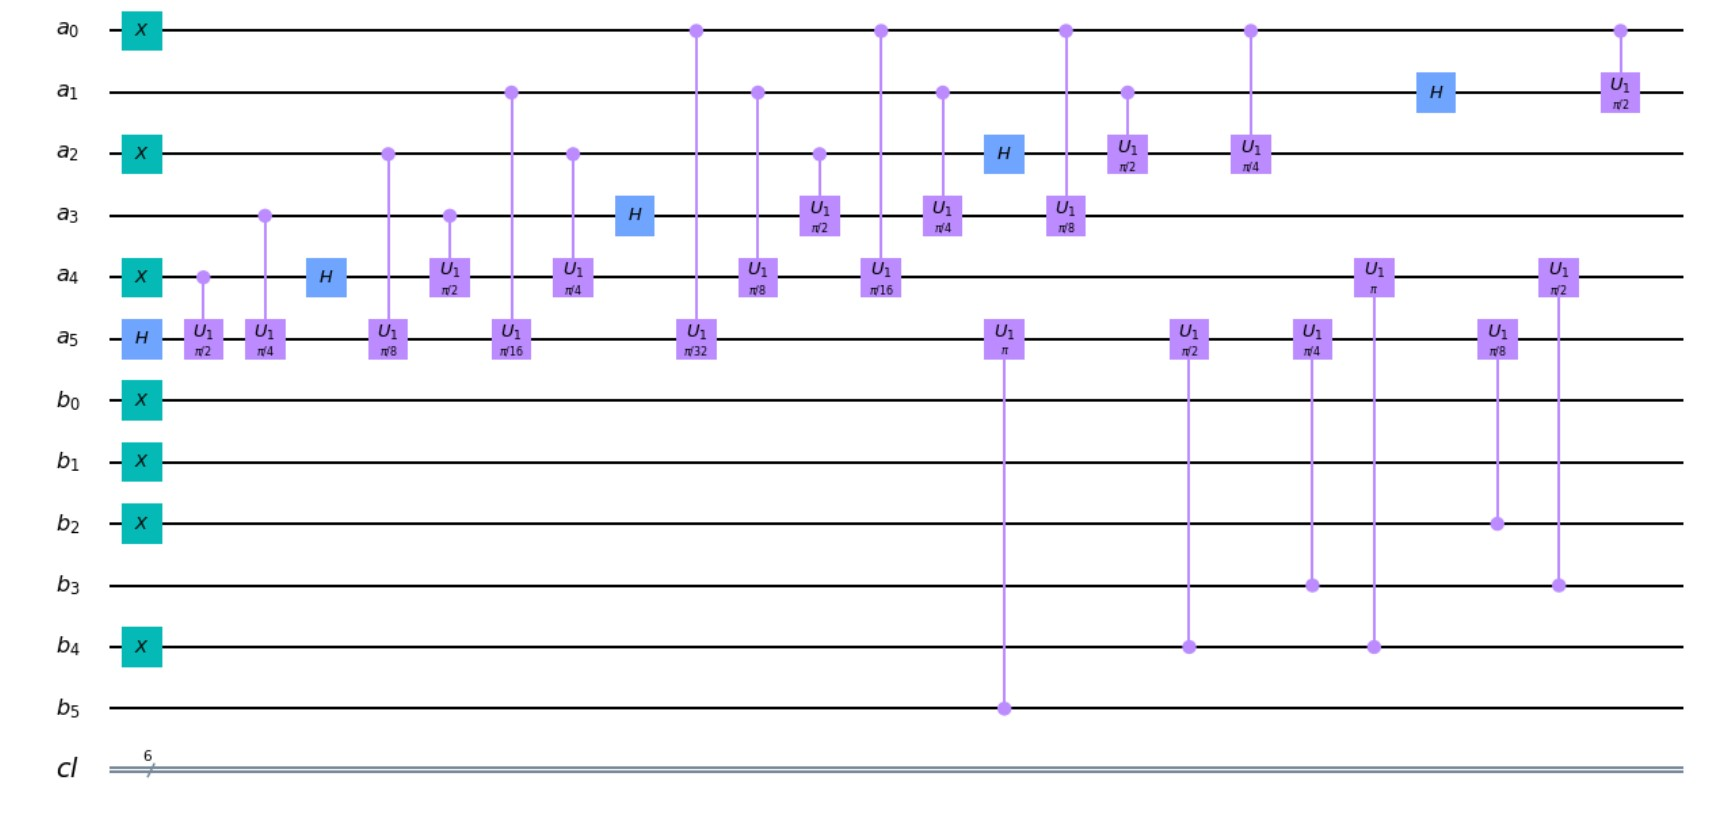
\includegraphics[width=14cm]{Thesis/images/Quantum_circuit_QFT_adder_1.jpg}
    \caption{Quantum circuit of QFT adder}
    \label{fig:figure12}
\end{figure*}

\begin{figure*}[htp]
    \centering
    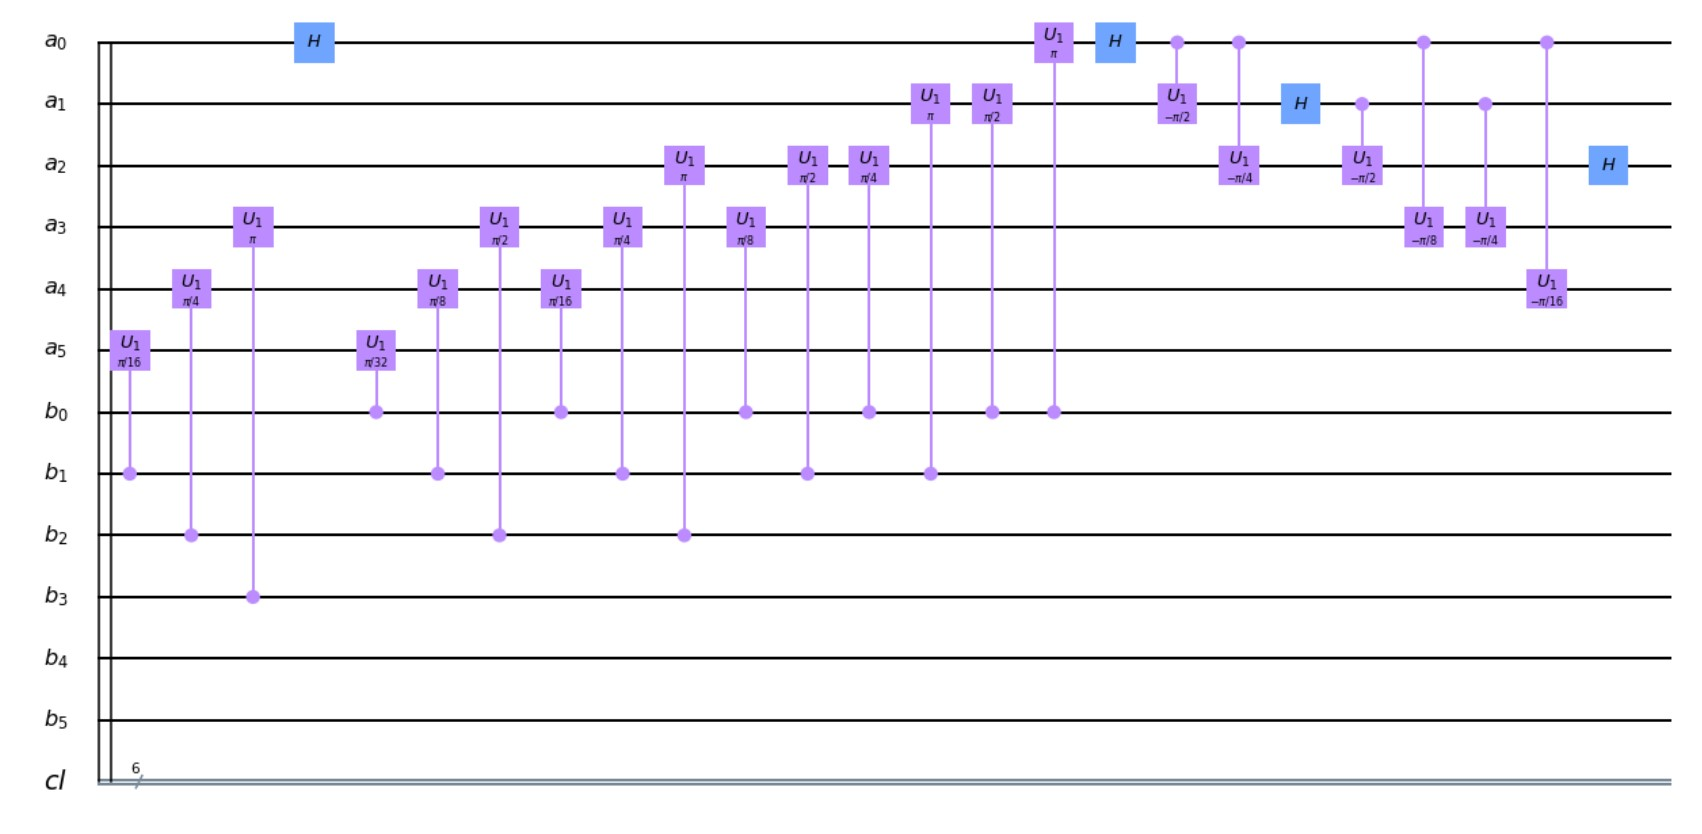
\includegraphics[width=14cm]{Thesis/images/Quantum_circuit_QFT_adder_2.jpg}
    \caption{Quantum circuit of QFT adder}
    \label{fig:figure13}
\end{figure*}

\begin{figure*}[htp]
    \centering
    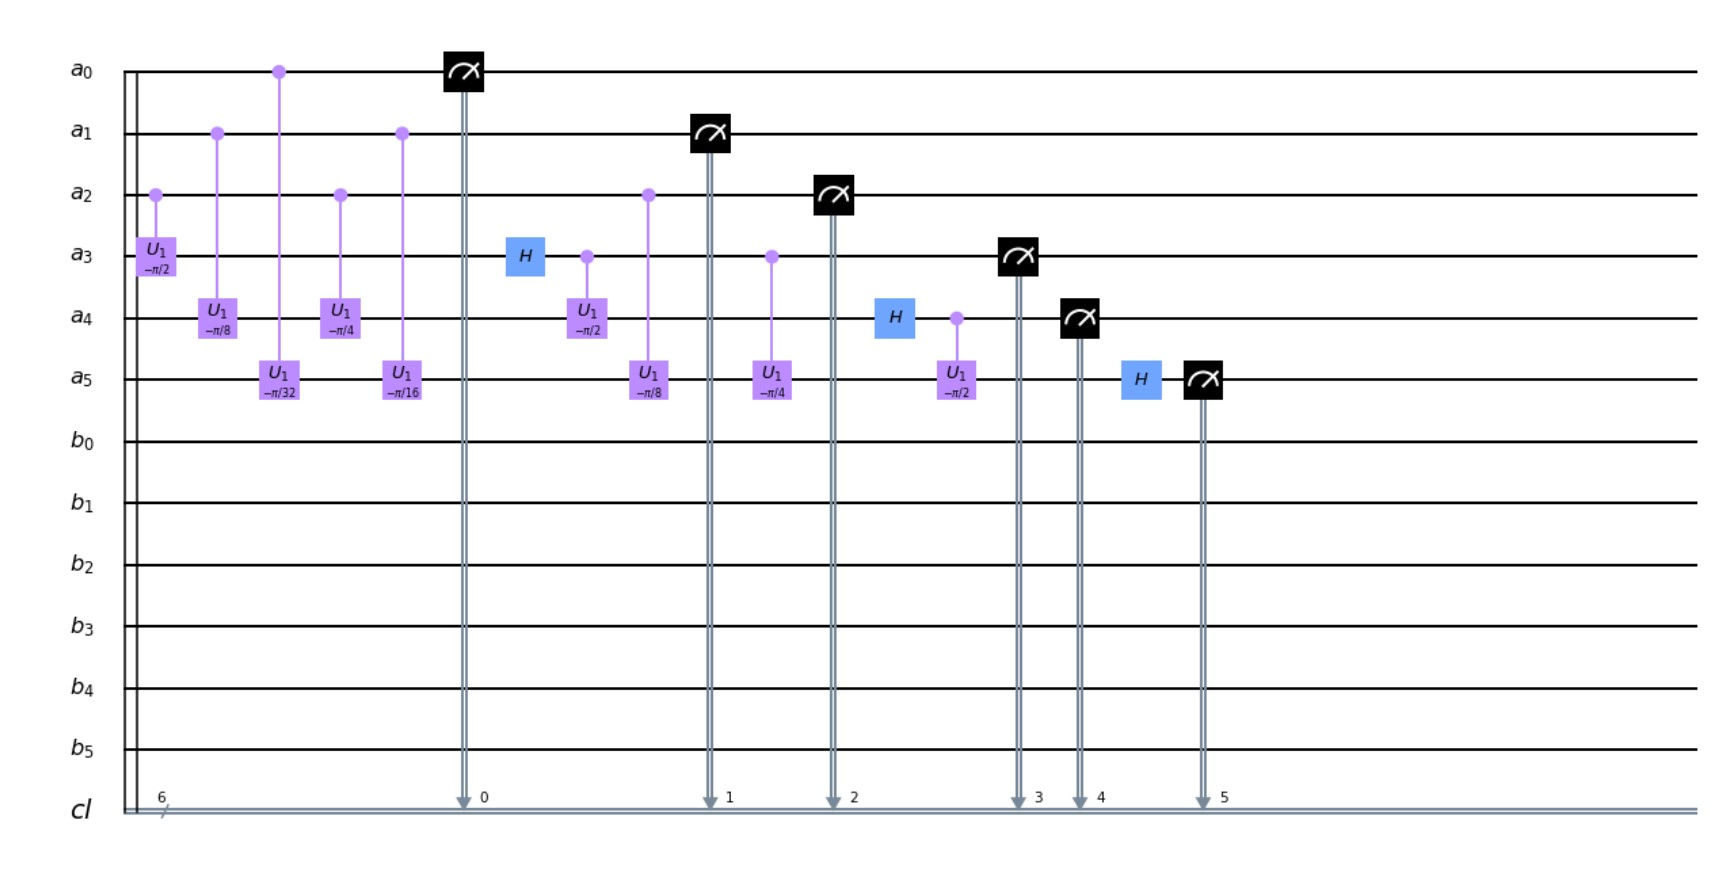
\includegraphics[width=14cm]{Thesis/images/Quantum_circuit_QFT_adder_3.jpg}
    \caption{Quantum circuit of QFT adder}
    \label{fig:figure14}
\end{figure*}


\newpage

\section{Multiplication using QFT adder}

Multiplication operation can be performed using repeated addition. This module was developed using QFT adder described in the previous section \cite{sashwat_multiplication}.

This multiplication module is designed for multiplying $p$ and $q$ and to calculate $\phi(n)$ in RSA crypto algorithm. This function takes two classical numbers as arguments since the generated prime number function returns classical number as an output and then loads these numbers into Quantum registers for further Quantum operations. To form a multiplication module, below procedure is followed:

•	Create a zero initialized accumulator.

•	Add the multiplicand to the accumulator.

•	Decrement the multiplier by one.

•	Repeat the last two steps until the multiplier becomes zero.

For Example, $13 * 3 = 39$ can be performed using the above rules as shown in Table \ref{table:table5}

\begin{table}[h]
\centering
\caption{Steps to perform multiplication}
\begin{tabular}{llll}
\hline
$Iteration$ &
$Multiplicand$ &
$Muliplier$ &
$Accumulator$ \\
\hline
0 &
1101 &
11 &
0 \\
1 &
1101 &
10 &
1101 \\
2 &
1101 &
1 &
11010 \\
3 &
1101 &
0 &
100111 \\
\hline
\end{tabular}
\label{table:table5}
\end{table}

\newpage
To decrement the multiplier, $factor$ was set to $-1$ in QFT adder to perform subtraction.

\begin{lstlisting}[escapeinside={(*}{*)}, language=Python]
def sub(reg_a, reg_b, circ, factor = -1):
    """
    Add two quantum registers reg_a and reg_b, and store the result 
    in reg_a.
    """
    pie = math.pi
    n = len(reg_a)
    # Compute the Fourier transform of register a
    for i in range(0, n):
        createInputState(circ, reg_a, n - (i+1), pie)
    # Add the two numbers by evolving the Fourier transform   
    # F((*$\psi$*)(reg_a))> to |F((*$\psi$*)(reg_a+reg_b))>
    for i in range(0, n):
        evolveQFTState(circ, reg_a, reg_b, n - (i+1), pie, factor)
    # Compute the inverse Fourier transform of register a
    for i in range(0, n):
        inverseQFT(circ, reg_a, i, pie)
\end{lstlisting}

\newpage
\begin{lstlisting}[escapeinside={(*}{*)}, language=Python]
def mul(multiplicand_in, multiplier_in):
    # Take two numbers as user input in binary form
    # multiplicand_in = input("Enter the multiplicand.")
    l1 = len(multiplicand_in)
    # multiplier_in = input("Enter the multiplier.")
    l2 = len(multiplier_in)
    # Make sure multiplicand_in holds the larger number
    if l2 > l1:
        multiplier_in, multiplicand_in = multiplicand_in, multiplier_in
        l2, l1 = l1, l2

    accumulator = QuantumRegister(l1 + l2)
    multiplicand = QuantumRegister(l1)
    multiplier = QuantumRegister(l2)
    d = QuantumRegister(1)
   
    cl_accumulator = ClassicalRegister(l1 + l2)
    cl_multiplier = ClassicalRegister(l2)
   
    circ_accumulator = QuantumCircuit(accumulator, multiplicand, cl_accumulator)
    circ_multiplier = QuantumCircuit(multiplier, d, cl_multiplier)
    circ_multiplier.x(d[0])
   
    for i in range(l1):
        if multiplicand_in[i] == '1':
            circ_accumulator.x(multiplicand[l1 - i - 1])
    for i in range(l2):
        if multiplier_in[i] == '1':
            circ_multiplier.x(multiplier[l2 - i - 1])
           
    multiplier_str = '1'
    while(int(multiplier_str) != 0):
        add(accumulator, multiplicand, circ_accumulator)
        sub(multiplier, d, circ_multiplier)
        circ_multiplier.measure(multiplier, cl_multiplier)
        result = execute(circ_multiplier, backend=Aer.get_backend('qasm_simulator'), shots=2).result().get_counts(circ_multiplier)
        multiplier_str = list(result.keys())[0]
   
    circ_accumulator.measure(accumulator, cl_accumulator)
    result = execute(circ_accumulator, backend=Aer.get_backend('qasm_simulator'), shots=2).result().get_counts(circ_accumulator)
    total = list(result.keys())[0]
    return total
\end{lstlisting}

\section{Montgomery Multiplication}	

The main advantage of Montgomery approach is that it avoids the division operation needed for modular multiplication\cite{alfred:paul:scott}. As it is implemented in FPGA in chapter 2, algorithm \ref{algorithm1} can be implemented for Quantum RSA using IBM's Qiskit. Different approaches have been tried to implement the algorithm in efficient way to make sure it performs better and uses lesser number of qubits, since qubits are limited in IBM Q as it is in early stages of development.

\newpage
As an initial step, length of $x$ input was measured and Quantum registers and Classical registers were assigned with extra bits as needed for the operation.

\begin{lstlisting}[language=Python]
# Measuring the length of x
n = len(x)

# Assigning Quantum registers for Quantum operation
x_reg = QuantumRegister(n+1)
y_reg = QuantumRegister(n+2)
y_reg_0 = QuantumRegister(1)
m_reg = QuantumRegister(n+2)
a_reg = QuantumRegister(n+2)
u_reg = QuantumRegister(n+1)
onecubit = QuantumRegister(1)

# Assigning classical registers to store our results from Quantum registers
a_cl_reg = ClassicalRegister(n+2)
u_cl_reg = ClassicalRegister(n+1)
cl_reg = ClassicalRegister(n+1)
one_cl_reg = ClassicalRegister(1)
\end{lstlisting}

Separate Quantum circuits was created for each sets of addition in the algorithm. This way of implementing circuits makes sure the performance is faster than if they are implemented in a single circuit. 

\newpage
\begin{lstlisting}[language=Python]
# creating seperate Quantum circuits for different operations to speedup the process
circ_u = QuantumCircuit(u_reg, y_reg_0, u_cl_reg)
circ_a = QuantumCircuit(a_reg, y_reg, m_reg, a_cl_reg, onecubit, one_cl_reg)
\end{lstlisting}

Inputs were loaded into Quantum registers using the below code snippet

\begin{lstlisting}[language=Python]
# Loading inputs to Quantum registers
for i in range(n):
    if y[i] == '1':
        circ_a.x(y_reg[n - i - 1])
for i in range(n):
    if m[i] == '1':
        circ_a.x(m_reg[n - i - 1])
\end{lstlisting}

Addition was performed using QFT adder in the intermediate steps of Montgomery modular multiplication. In order to take decision according to the addition results, qubits were measured in each iteration. 

\begin{lstlisting}[language=Python]
for i in range(n):
    if x[n - i - 1] == '1':            
        add(u_reg, y_reg_0, circ_u)
    circ_u.measure(u_reg[0], u_cl_reg[0])  
    result = execute(circ_u,backend=Aer.get_backend('qasm_simulator'), shots=1).result().get_counts(circ_u)
    measure_u = int((list(result.keys())[0]))
    print('measure_u: ', measure_u)
   
    if x[n - i - 1] == '1':
        add(a_reg, y_reg, circ_a)
    if measure_u == 1:
        add(a_reg, m_reg, circ_a)
    rshift(circ_a, a_reg, n + 2, onecubit)
    circ_a.measure(a_reg, a_cl_reg)
    circ_a.measure(onecubit, one_cl_reg)
    result = execute(circ_a,backend=Aer.get_backend('qasm_simulator'), shots=1).result().get_counts(circ_a)
    total = list(result.keys())[0]    
    measure_a = total[2:]
    print(measure_a)
   
    measure_onecubit = int(total[0])
    if measure_onecubit == 1:
        circ_a.x(onecubit)    
   
    # loading a0 to u0
    if measure_a[n + 1] == '1':
        if measure_u == 0:
            circ_u.x(u_reg[0])
    else:
        if measure_u == 1:
            circ_u.x(u_reg[0])
\end{lstlisting}

As a final step, if calculated answer is greater than the ‘m’ value, then it is subtracted from ‘m’ to get the final answer. Else, the obtained answer is the final result. 

\begin{lstlisting}[language=Python]
if (int(measure_a) >= int(m)):
    sub(a_reg, m_reg, circ_a)
   
circ_a.measure(a_reg, a_cl_reg)
result = execute(circ_a,backend=Aer.get_backend('qasm_simulator'), shots=1).result().get_counts(circ_a)
total = list(result.keys())[0]    
final_a = total[2:]
print(final_a)
\end{lstlisting}

Results of Montgomery multiplication is shown in figure \ref{fig:figure15}. This function outputs values in montgomery domain as they will be further used in exponentiation operation.

\begin{figure*}[htp]
    \centering
    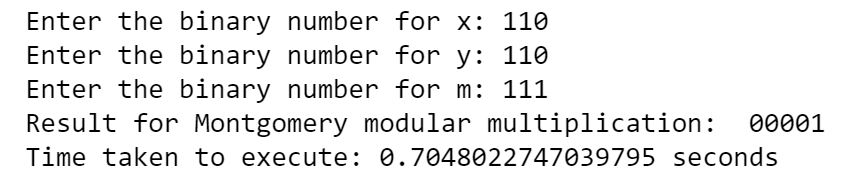
\includegraphics[width=14cm]{Thesis/images/Mont_multiplication_quantum.JPG}
    \caption{Results for Montgomery modular multiplication using Qiskit}
    \label{fig:figure15}
\end{figure*}


\section{Montgomery Exponentiation}

Once modular multiplication is performed using Montgomery technique, the same can be used multiple times with different parameters in order to achieve exponentiation operation \cite{alfred:paul:scott}. Refer figure \ref{fig:figure8} for internal details of Montgomery Exponentiation algorithm.

\newpage
\begin{lstlisting}[language=Python]
def Mont_Exp(x, e, m):
    L = len(m)
    
    # R calculation
    R = 2**L

    # R mod m or Initial A calculation:
    R_mod_m = R % int(m,2) #int('string', base)
    A = str(R_mod_m)
    A = str(bin(int(A))[2:]).zfill(L) 

    # R^2 mod m calculation
    R_square_mod_m = str(((R**2) % int(m,2)))
    T = len(e)
    R_square_mod_m = str((bin(int(R_square_mod_m))[2:])).zfill(L)
    
    # writing input x in montgomery domain called x_dash
    x_dash = Mont_Mul(x, R_square_mod_m, m)
   
    for i in range(0,T):
        if (len(A) > L):
            A = A[2:L+2]
        A = Mont_Mul(A, A, m)
        if e[i] == '1':
            A = Mont_Mul(A[2:L+2], x_dash[2:L+2], m)
            

    A = Mont_Mul(A[2:L+2], '1'.zfill(L), m)
    return A
\end{lstlisting}

\begin{figure*}[htp]
    \centering
    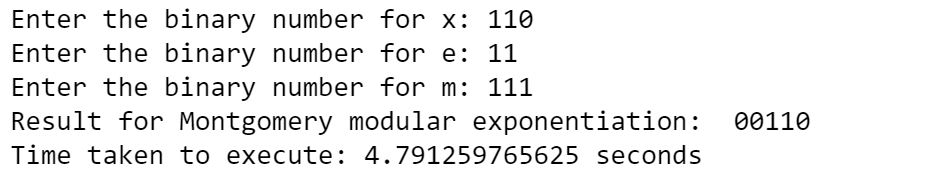
\includegraphics[width=14cm]{Thesis/images/Mont_exponentiation_quantum.JPG}
    \caption{Results for Montgomery modular exponentiation using Qiskit}
    \label{fig:figure16}
\end{figure*}

\section{Modular Inverse}	

Modular inverse is an essential operation to find the private key $d$ for RSA decryption. Montgomogery modular exponentiation can be used to calculate modular inverse only if the modular value is an odd integer. Since, even modular integers are involved in finding a private key, exponentiation algorithm can't be used. This demands a separate algorithm to calculate modular inverse. The disadvantage of using a conventional GCD algorithms is that, it requires multiple precision division operations \cite{alfred:paul:scott}. Binary extended GCD algorithm eliminates this requirement at the expense of more iterations.
$271^{-1}\,mod\,383 = 106$ is an example for modular inverse calculation, which is shown in figure \ref{fig:figure19}

\begin{figure*}[htp]
    \centering
    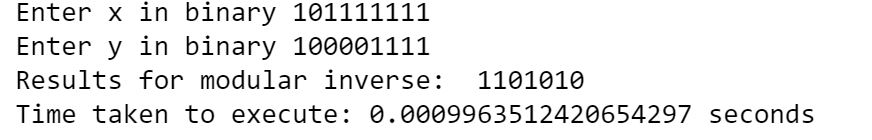
\includegraphics[width=14cm]{Thesis/images/Mod_inverse_quantum.JPG}
    \caption{Results for Binary Extended GCD algorithm for modular inverse}
    \label{fig:figure19}
\end{figure*}

\section{Encryption and Decryption}	

Since Montgomery multiplication, exponentiation and modular inversion are implemented as efficient functions, they can be used to perform encryption and decryption for RSA algorithm. $C$ denotes encrypted/cipher text and $M$ denotes decrypted/original text.

\begin{lstlisting}[language=Python]
d = Mod_Inv(PhiofN,e)

# Getting message from User
M = input("Enter the message in binary")

# Encryption process or calculating cipher text
C = Mont_Exp(M, e, N)
print('Encrypted text: ', C)

# Decryption process or calculating original text
M = Mont_Exp(C, d, N)
print('Original Text: ', M)
\end{lstlisting}

\newpage
\begin{figure*}[htp]
    \centering
    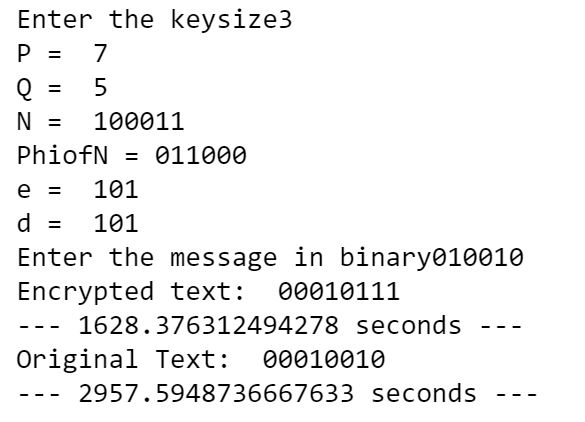
\includegraphics[width=14cm]{Thesis/images/Encryption_decryption_quantum.JPG}
    \caption{Results for RSA Encryption and Decryption using Qiskit}
    \label{fig:figure20}
\end{figure*}


\section{Conclusion}

% it can be used for max 3 bits, because of quantum bits limitation. with advancement in quantum computers with more bits, the same algorithm can be used for n bits, proving this research to be scalable approach. It is successfully implemented in FPGA and Quantum computer using Qiskit to analyze its vulnerability. its vulnerable to shor's algorithm.




%
% ---- Bibliography ----
%
\begin{thebibliography}{7}
%

\addcontentsline{toc}{chapter}{{Bibiliography}}

\bibitem{gary}
Gary C. Kessler: An Overview of Cryptography, Handbook on Local Area Networks, Auerbach (1998).

\bibitem{nist}
NIST: Post-Quantum Cryptography, https://csrc.nist.gov/Projects/Post-Quantum-Cryptography (2019).

\bibitem{nirmala:praveena}
S. Nirmala, R. Praveena: Implementation of efficient modular bypass multiplier logic in rsa cryptographic processor, International Conference and Workshop on Electronics and
Telecommunication Engineering (2016).

\bibitem{yan:wu:zheng:xie}
X. Yan, G. Wu, D. Wu, F. Zheng, X. Xie: An implementation of montgomery modular multiplication on fpgas, 2013 International Conference on Information Science and Cloud Computing (2013).

\bibitem{rahman:rokon}
M. Rahman, I. R. Rokon: Efficient hardware implementation of rsa cryptography, 2009 3rd International Conference on Anti-counterfeiting, Security, and Identification in Communication (2009).  

\bibitem {mario:guillermo:francisco}
Mario Alberto García Martínez, Guillermo Morales Luna, Francisco Rodríguez Henríquez: Hardware Implementation of the Binary Method for Exponentiation in GF(2m). Proceedings of the Fourth Mexican International Conference on Computer Science, Tlaxcala, Mexico, Mexico (2003).

\bibitem {hans:nils:sheueling:vipul:leonard}
Hans Eberle, Nils Gura, Sheueling Chang Shantz, Vipul Gupta, Leonard Rarick: A public-key cryptographic processor for RSA and ECC, Proceedings. 15th IEEE International Conference on Application-Specific Systems, Architectures and Processors, Galveston, TX, USA (2004).

\bibitem {sushanta:manoranjan}
Sushanta Kumar Sahu, Manoranjan Pradhan: Implementation of Modular multiplication for RSA Algorithm. International Conference on Communication Systems and Network Technologies, Katra, Jammu, India (2011).

\bibitem {manish:amit:aakanksha:abhinav}
Manish Bansal, Amit Kumar, Aakanksha Devrari, Abhinav Bhat: Implementation of Modular exponentiation using Montgomery algorithms. International Journal of Scientific and Engineering Research, Volume 6, Issue 11 (2015).

\bibitem {nadia:luiza}
Nadia Nedjah, Luiza De Macedo Mourelle: Hardware Architecture for the Montgomery Modular Multiplication. International Conference on Information Technology Coding and Computing, Las Vegas, NV, USA (2004).

\bibitem {alfred:paul:scott}
Alfred J. Menezes, Paul C. van Oorschot, Scott A. Vanstone: Handbook of Applied Cryptography. 5th Edition (2001).

\bibitem{kumar:kumar:parthibane}
S. P. kumar, K. kumar, B.Partibane: Efficient modular exponentiation architectures for rsa algorithm, International Journal of Engineering Research in Electronic and Communication Engineering (IJERECE) Vol 3, Issue 5 (2016).

\bibitem{quantum_computing_medium}
Jlspursfan: Quantum Computing, https://medium.com/swlh/quantum-computing-1d40d4ed43b2 (2019).

\bibitem{sashwat_simple_adder}
Sashwat Anagolum: Arithmetic on Quantum Computers - Addition, https://medium.com/@sashwat.anagolum/arithmetic-on-quantum-computers-addition-7e0d700f53ae (2018).

\bibitem{quantum_gates_book_ibm}
Abraham Asfaw, Luciano Bello, Yael Ben-Haim, Sergey Bravyi, Lauren Capelluto, Almudena Carrera Vazquez, Jack Ceroni, Jay Gambetta, Shelly Garion, Leron Gil, Salvador De La Puente Gonzalez, David McKay, Zlatko Minev, Paul Nation, Anna Phan, Arthur Rattew, Javad Shabani, John Smolin, Kristan Temme, Madeleine Tod, James Wootton: Learn Quantum Computation using Qiskit (2019).

\bibitem{sashwat_fast_adder}
Sashwat Anagolum: Arithmetic on Quantum Computers - Addition, Faster, https://medium.com/@sashwat.anagolum/qftaddition-ce0a0b2bc4f4 (2018).

\bibitem{sashwat_multiplication}
Sashwat Anagolum: Arithmetic on Quantum Computers - Multiplication, https://medium.com/@sashwat.anagolum/arithmetic-on-quantum-computers-multiplication-4482cdc2d83b (2018).









\end{thebibliography}

\end{document}
